\chapter{Implementasi dan Pengujian}
\label{chap:implementasi_dan_pengujian}

Bab ini terdiri atas implementasi, pengujian, dan masalah yang dihadapi. Pada bagian implementasi dijelaskan mengenai lingkungan implementasi dan hasil dari implementasi. Pada bagian pengujian berisi hasil dari pengujian. Pada bagian masalah yang dihadapi akan dijelaskan masalah-masalah menarik yang dihadapi pada saat implementasi. 

\section{Implementasi}
\label{sec:implementasi}

Implementasi ini dilakukan dengan menggunakan \textit{Game Engine} Unity. Implementasi dilakukan pada satu buah laptop, dan aplikasi dijalankan pada tiga buah \textit{smartphone} Android. 

\subsection{Lingkungan Implementasi}
\label{ssec:lingkungan_implementasi_dan_pengujian}

Berikut adalah spesifikasi laptop yang digunakan untuk implementasi:
\begin{enumerate}
    \item Processor : AMD A10-5750M Quad-core 2.5 - 3.5 Ghz
    \item RAM : 8GB (7.21 Usable)
    \item VGA : AMD Radeon HD 8650G + HD 8670M Dual Graphics
    \item Sistem Operasi : Windows 10 64-bit
    \item Versi Unity : 5.5.1f1 Personal Edition
    \item Google VR SDK for Unity : 1.1 
\end{enumerate}

Berikut adalah spesifikasi perangkat \textit{smartphone} android yang digunakan untuk implementasi:
\begin{enumerate}
    \item Processor : Qualcomm Snapdragon 625 Octa-core 2.0 GHz Cortex-A53
    \item Sistem Operasi : Android OS 6.0 (Marshmallow)
    \item Sensor-sensor : Accelerometer, gyro, proximity, compass, barometer
\end{enumerate}

\subsection{Hasil Implementasi}

Hasil Implementasi ini adalah aplikasi permainan VR berbasis Android yang menggunakan Game Engine Unity. Aplikasi ini dapat di \textit{install} dengan menggunakan \textit{Package Installer} yang berekstensi file ".apk" pada Android.

\begin{enumerate}
    \item \textbf{Aplikasi saat pertama kali terbuka.}\\
    Pada saat pertama kali dijalankan permainan akan langsung dimulai (Gambar \ref{fig:aplikasi_mulai}). Jika perangkat tidak memiliki sensor Gyroscope, aplikasi akan menampilkan \textit{pop-up} (Gambar \ref{fig:no_gyroscope}) yang menunjukkan bahwa perangkat ini tidak dapat menjalankan aplikasi ini. Tombol 'X' pada pojok kiri atas akan selalu ada pada permainan ini dan berguna sebagai tombol untuk keluar dari permainan.
    
    \begin{figure}[htbp]
    \centering
    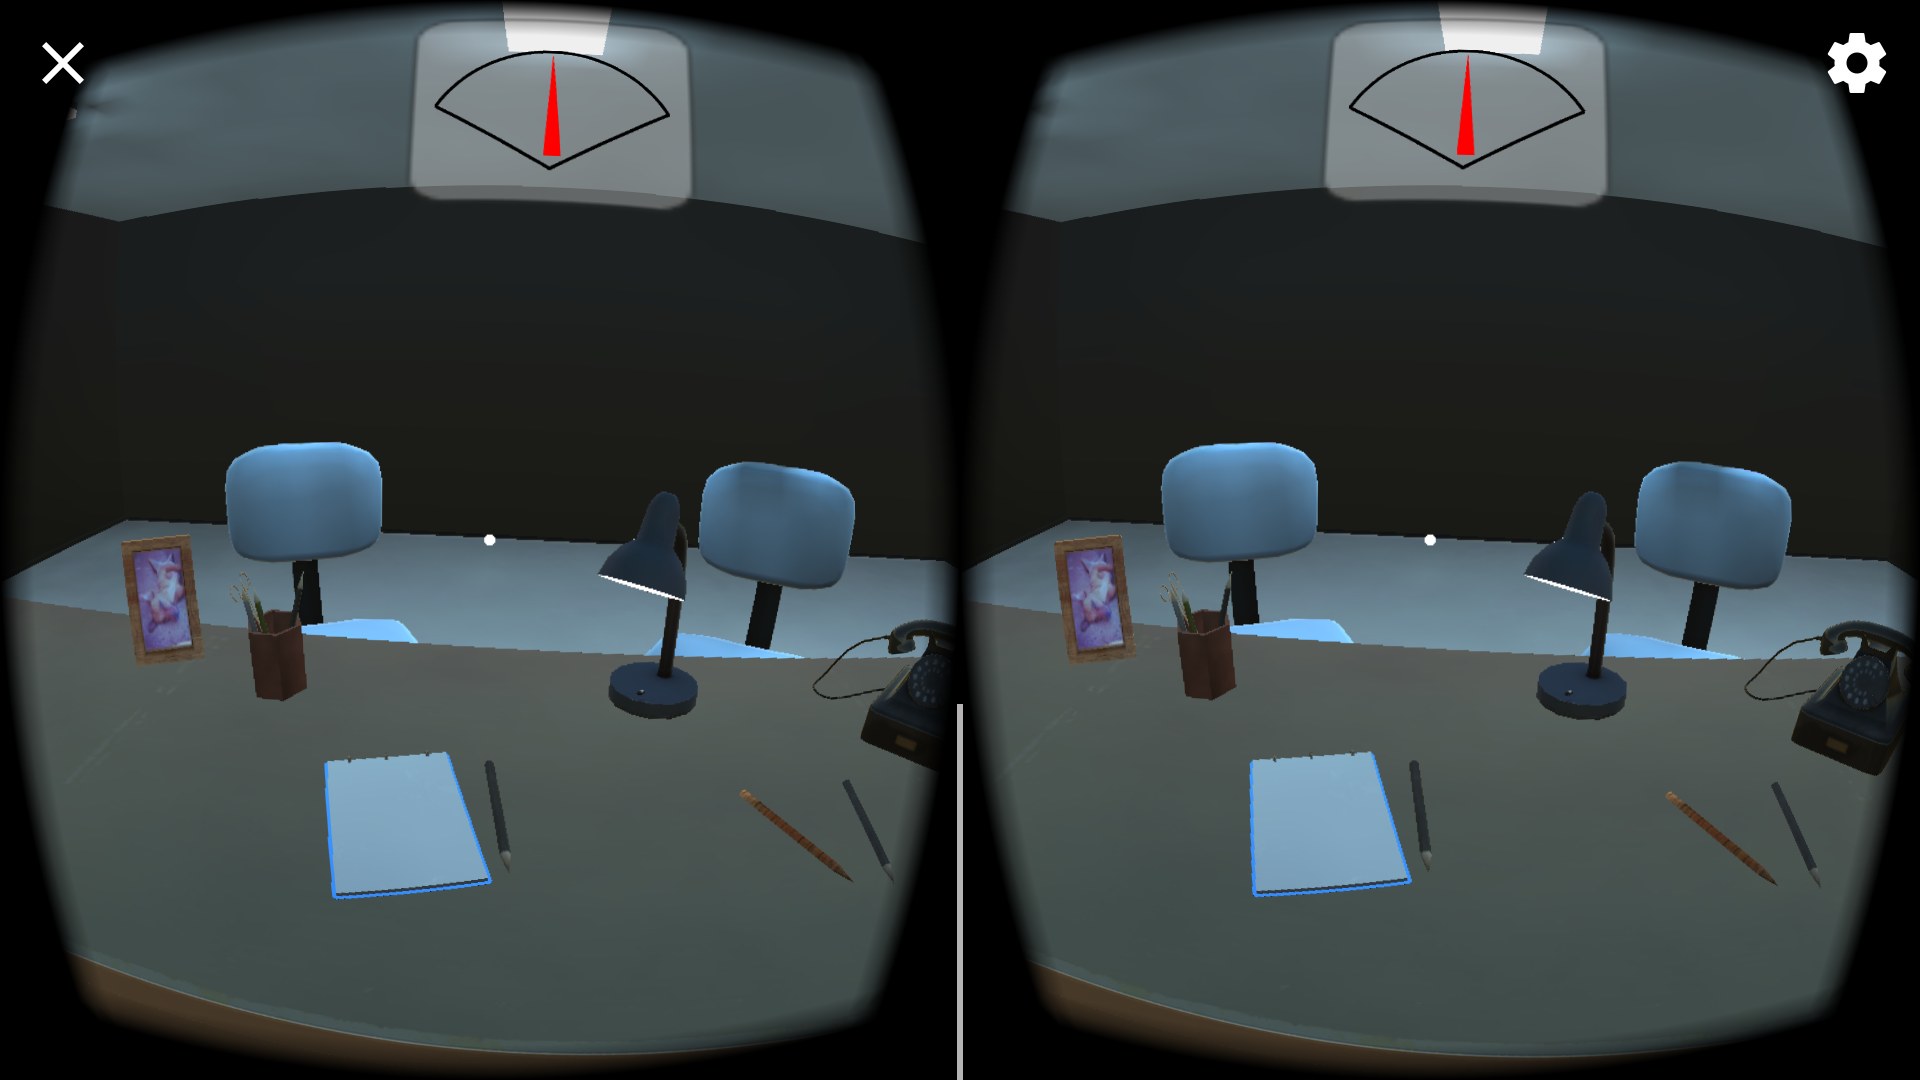
\includegraphics[scale=0.23]{Gambar/screenshot-aplikasi/aplikasi-mulai.png}
    \caption{Tampilan ketika aplikasi baru dimulai.} 
    \label{fig:aplikasi_mulai}
    \end{figure}
    
    \begin{figure}[htbp]
    \centering
    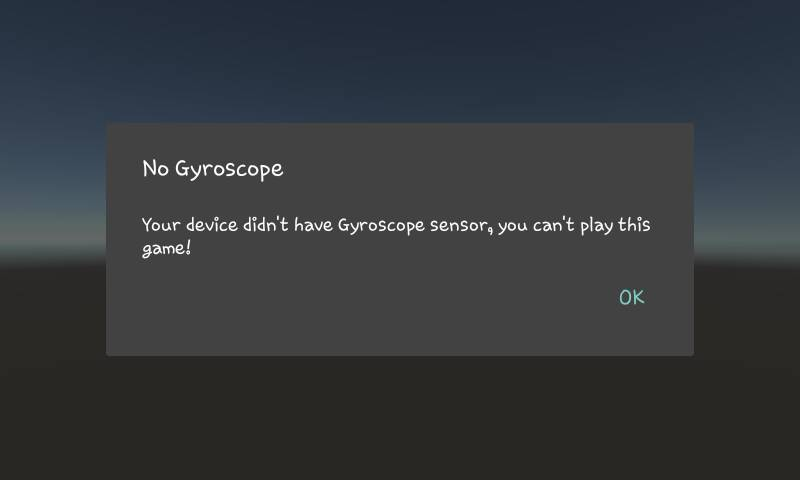
\includegraphics[scale=0.3]{Gambar/screenshot-aplikasi/no-gyroscope.jpg}
    \caption{Tampilan ketika perangkat tidak memiliki sensor Gryoscope.} 
    \label{fig:no_gyroscope}
    \end{figure}
    
    \item \textbf{Aplikasi saat muncul notifikasi.}\\
    Ketika ada notifikasi, akan muncul tanda seru (!) di atas benda yang memiliki notifikasi seperti pada Gambar \ref{fig:ss_notifikasi}.
    
    \begin{figure}[htbp]
    \centering
    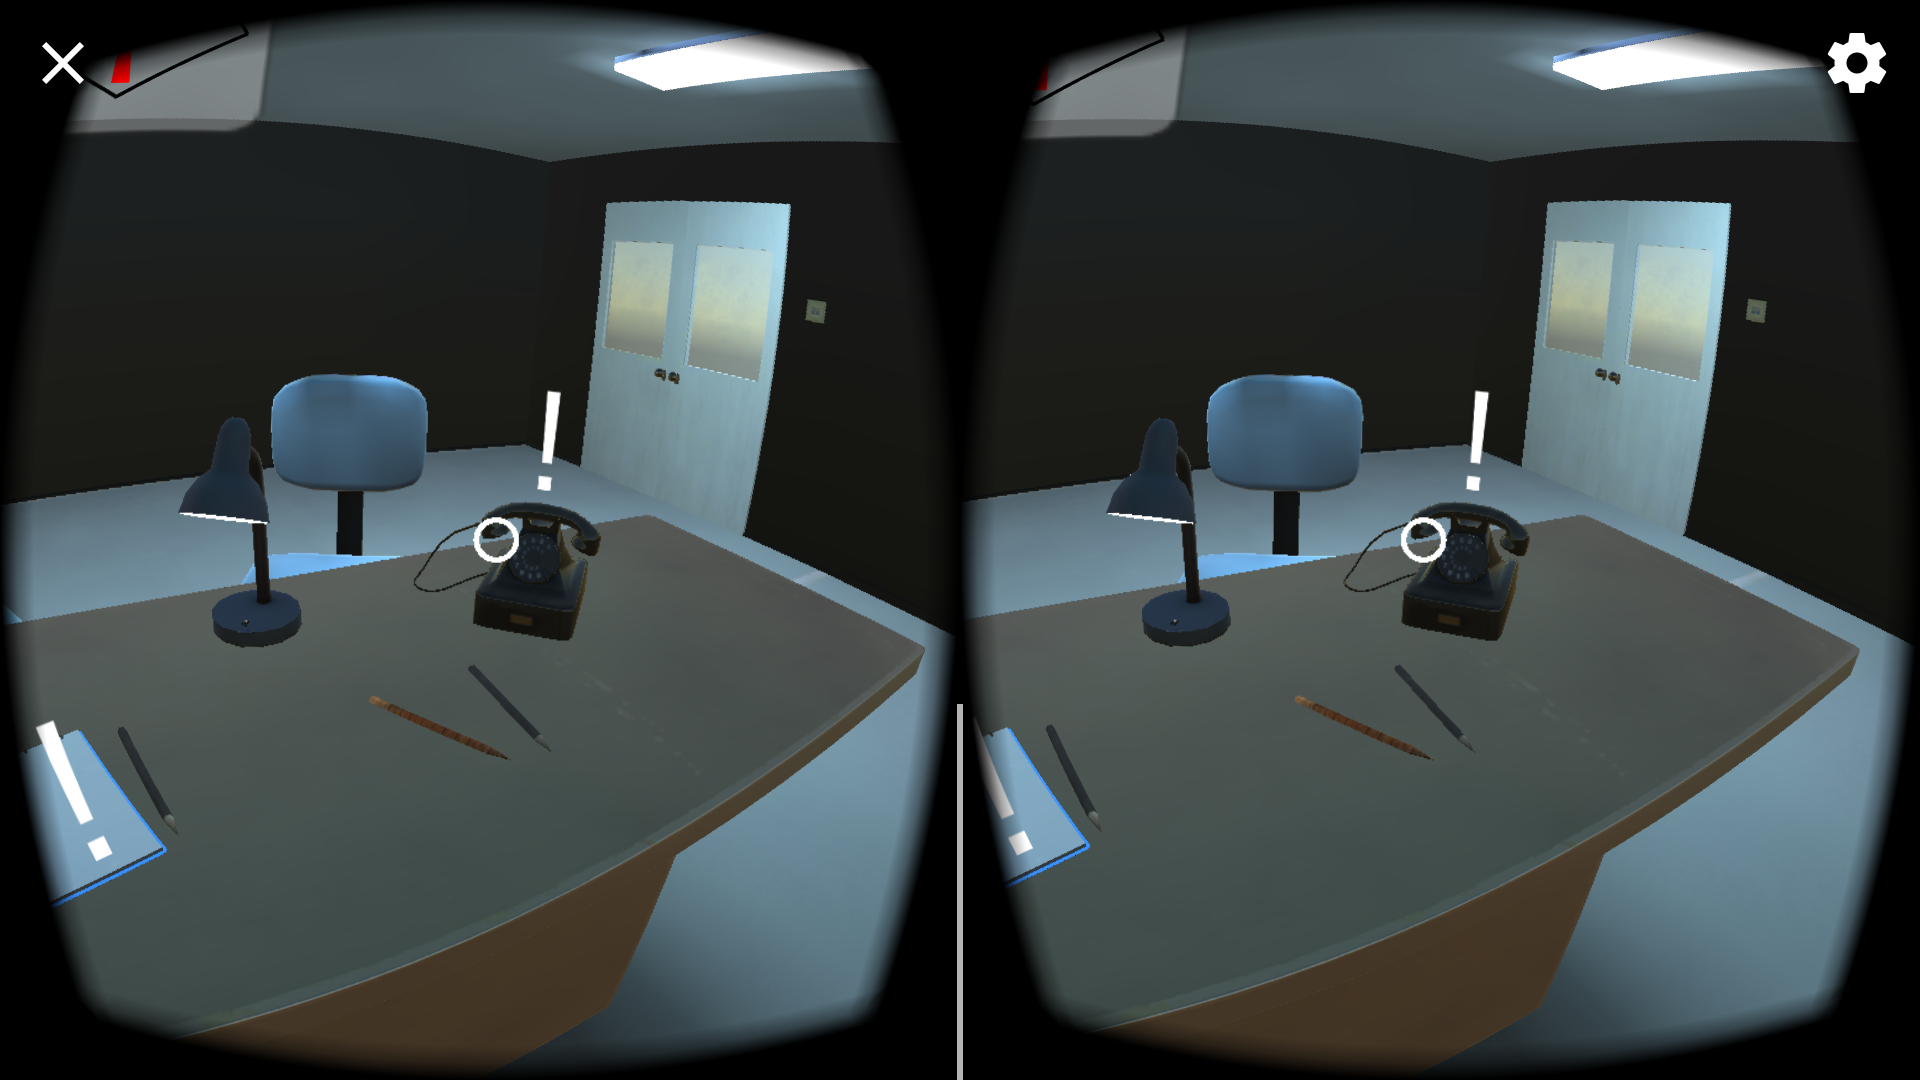
\includegraphics[scale=0.23]{Gambar/screenshot-aplikasi/muncul-notifikasi.png}
    \caption{Tampilan ketika notifikasi muncul.} 
    \label{fig:ss_notifikasi}
    \end{figure}
    
    \item \textbf{Aplikasi saat memunculkan pertanyaan.}\\
    Ketika pengguna sudah memilih suatu notifikasi yang muncul, akan muncul jendela pertanyaan di atas benda yang dipilih (Gambar \ref{fig:ss_pop_up}). 
    
    \begin{figure}[htbp]
    \centering
    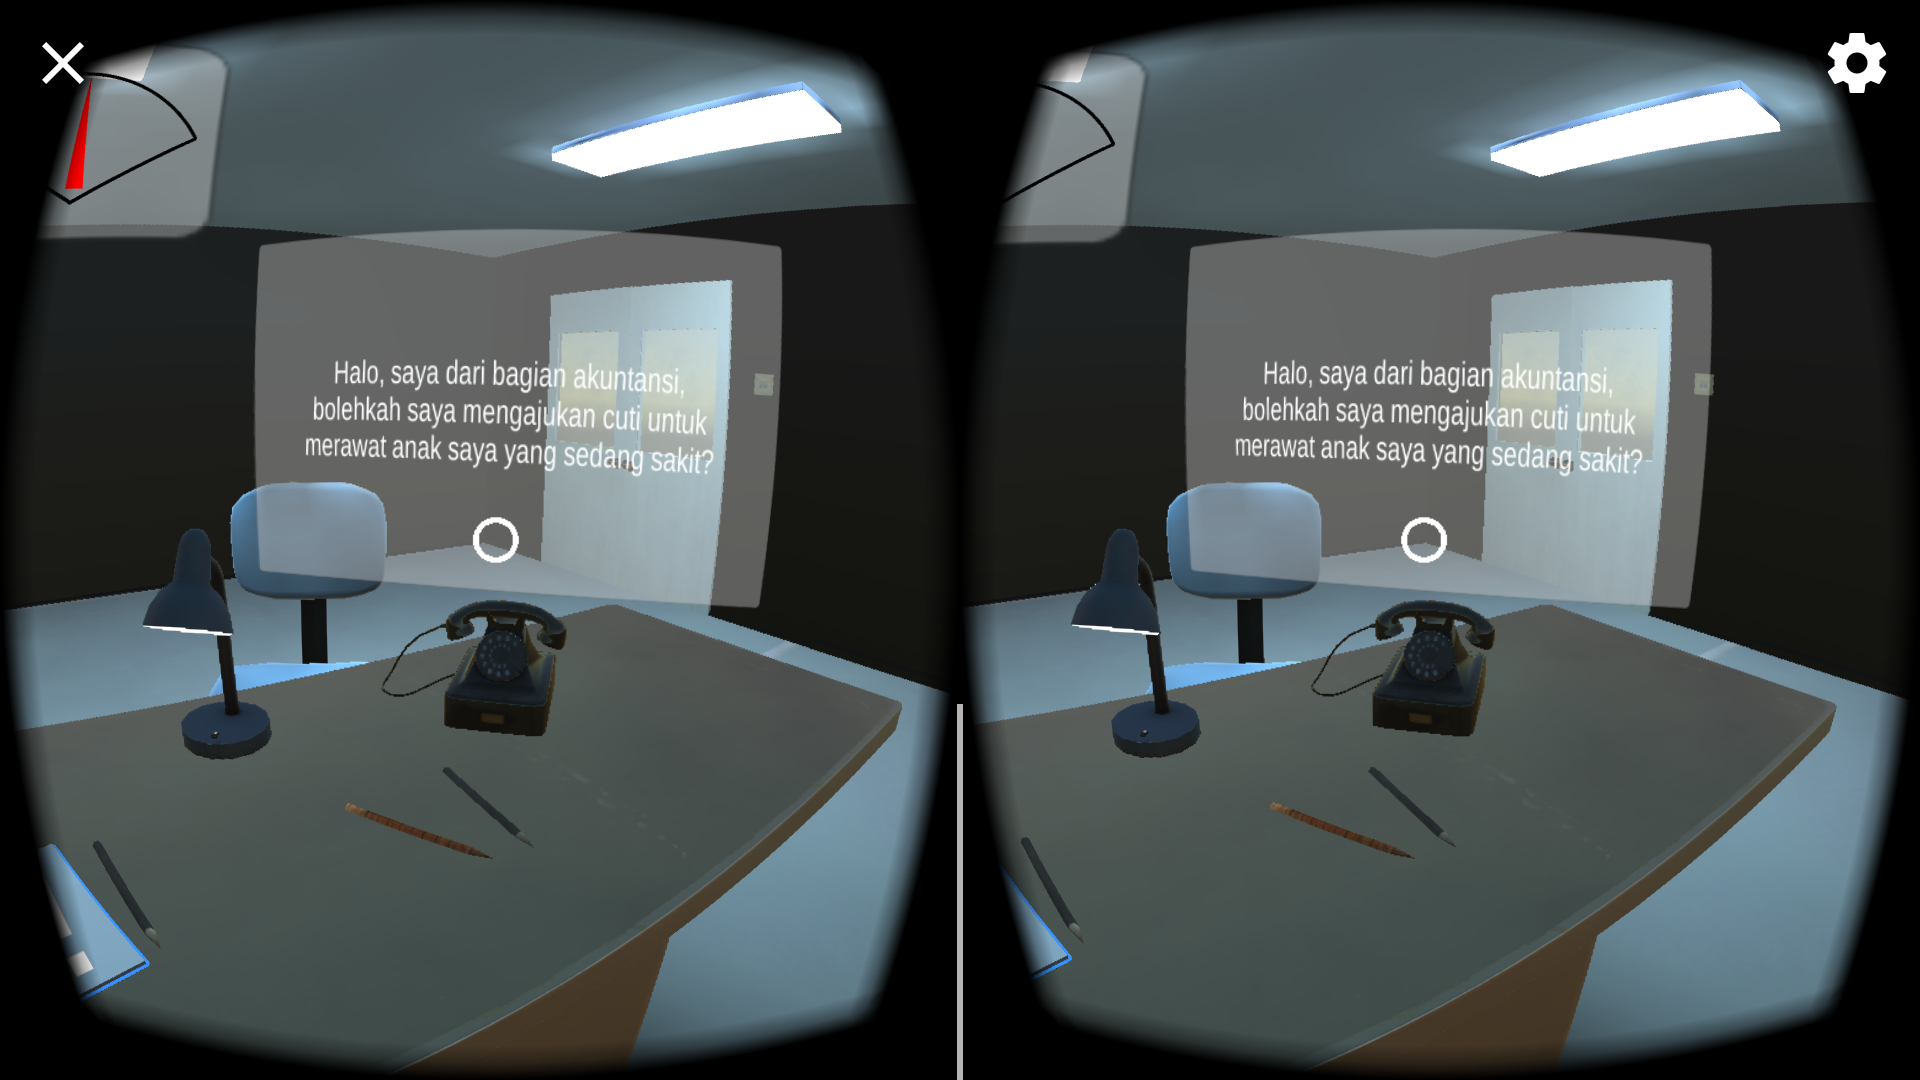
\includegraphics[scale=0.23]{Gambar/screenshot-aplikasi/pop-up.png}
    \caption{Tampilan ketika \textit{pop-up} pertanyaan muncul.} 
    \label{fig:ss_pop_up}
    \end{figure}
    
    \item \textbf{Aplikasi setelah memberikan respons mengangguk atau menggeleng.}\\
    Ketika pengguna mengangguk pada saat pertanyaan diberikan, tulisan pada panel pertanyaan akan berubah menjadi kata "YES"(Gambar \ref{fig:ss_pengguna_mengangguk}) dan "NO" ketika pengguna menggeleng (Gambar \ref{fig:ss_pengguna_menggeleng}).
    
    \begin{figure}[htbp]
    \centering
    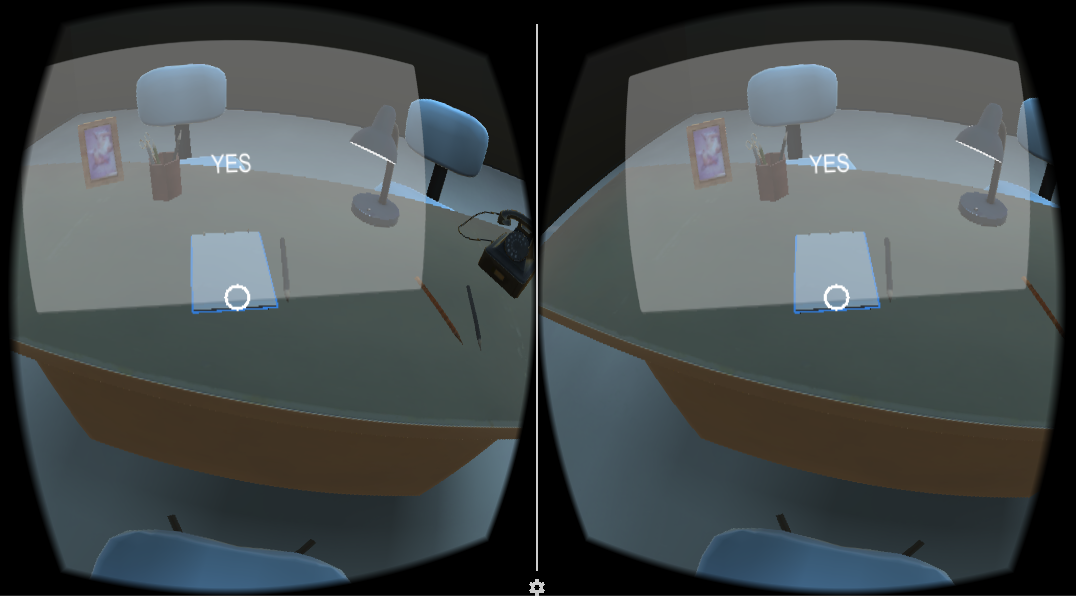
\includegraphics[scale=0.53]{Gambar/screenshot-aplikasi/pengguna-mengangguk.png}
    \caption{Tampilan setelah pengguna mengangguk.} 
    \label{fig:ss_pengguna_mengangguk}
    \end{figure}
    
    \begin{figure}[htbp]
    \centering
    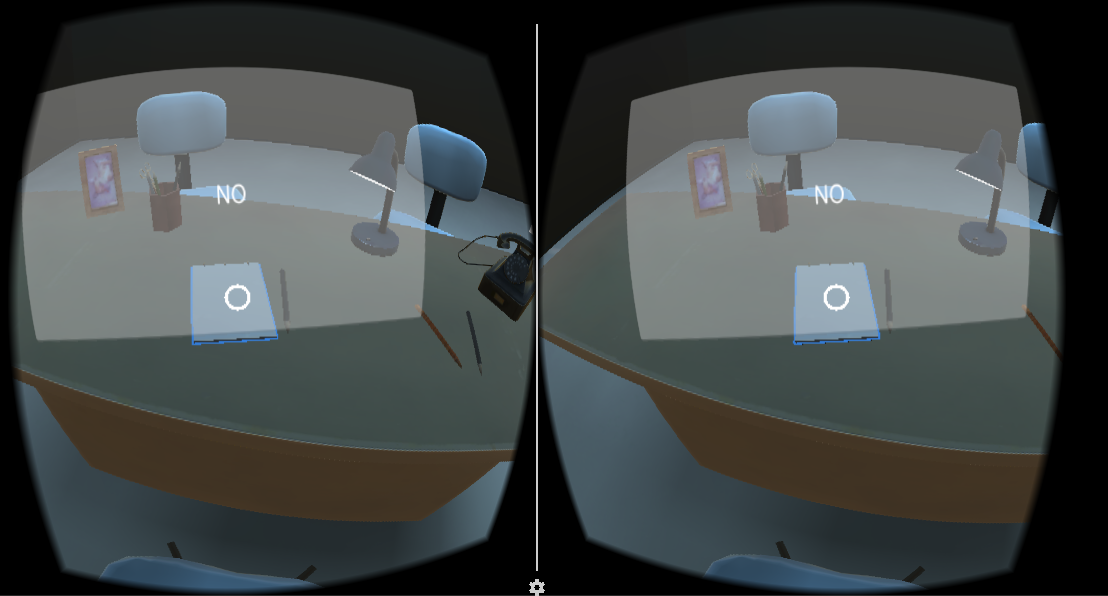
\includegraphics[scale=0.53]{Gambar/screenshot-aplikasi/pengguna-menggeleng.png}
    \caption{Tampilan setelah pengguna menggeleng.} 
    \label{fig:ss_pengguna_menggeleng}
    \end{figure}
    
    \item \textbf{Aplikasi ketika pemain kalah dalam permainan tersebut.}
    Ketika pengguna kalah, maka akan muncul tulisan "Game Over!" di depan pandangan pengguna (Gambar \ref{fig:ss_game_over}). Tulisan ini akan mengikuti pergerakan kepala pengguna. Jika pengguna menarik/menekan tombol pada Google Cardboard, permainan akan diulang menjadi kondisi awal.
    
    \begin{figure}[htbp]
    \centering
    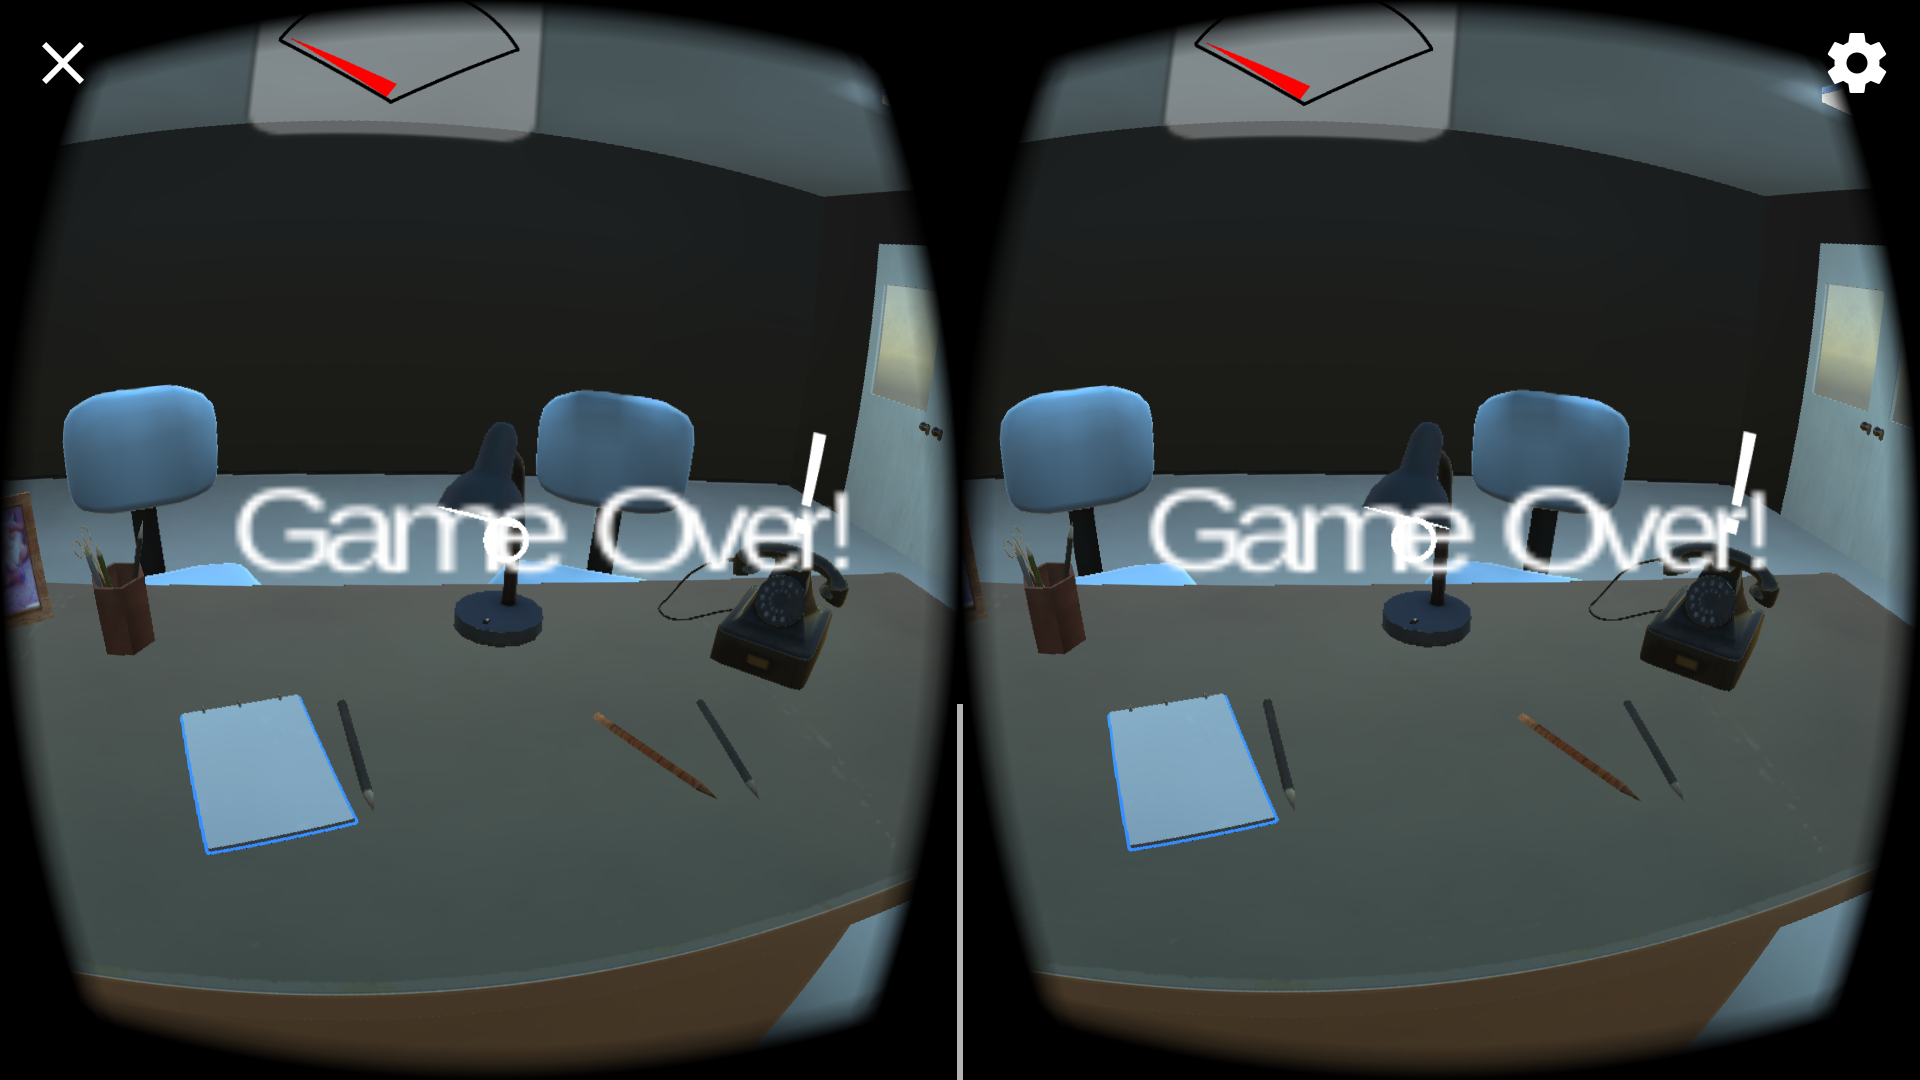
\includegraphics[scale=0.23]{Gambar/screenshot-aplikasi/game-over.png}
    \caption{Tampilan setelah permainan usai.}
    \label{fig:ss_game_over}
    \end{figure}
    
\end{enumerate}

\section{Pengujian}

Pengujian dilakukan dengan menggunakan dua buah metode yaitu pengujian fungsional dan pengujian eksperimental. Pengujian fungsional bertujuan untuk menguji fungsi-fungsi yang disediakan pada aplikasi. Pengujian Eksperimental bertujuan untuk menguji pengalaman pengguna dalam menggunakan aplikasi ini.

\subsection{Pengujian Fungsional}

Pengujian Fungsional ini dilakukan dengan mencoba menjalankan aplikasi pada perangkat-perangkat yang berbeda spesifikasi-nya. Tabel \ref{tab:tabel_perangkat_yang_digunakan} merupakan daftar perangkat-perangkat \textit{smartphone} Android yang di gunakan saat Implementasi

\begin{table}[]
    \centering
    \begin{tabular}{|p{1cm}||p{4cm}|p{4cm}|p{4cm}|}
    \hline\\
    \hline
       No  & Processor & Sistem Operasi & Sensor-sensor \\
    \hline
        1 &  Exynos Dual-core 1.4 GHz Cortex-A9 & Android OS v4.1.2 (Jelly Bean) & Accelerometer, gyro, proximity, compass, barometer\\
    \hline
        2 &  Qualcomm Snapdragon 800 Quad-core 2.3 GHz Krait 400 & Android OS v6.0 (Marshmallow) & Accelerometer, gyro, proximity, compass, barometer\\
    \hline
        3 &  Qualcomm Snapdragon 625 Octa-core 2.0 GHz Cortex-A53 & Android OS v6.0 (Marshmallow) & Fingerprint (rear-mounted), accelerometer, gyro, proximity, compass\\
    \hline
        4 &  Quad-core 1.2 GHz Cortex-A7 &  Android OS v4.4 (KitKat) & Accelerometer, proximity\\
    \hline
        5 &  1.3 GHz octa-core CPU, MediaTek Helio X10 MT6753 chipset & Android OS v6.0 (Marshmallow) & Accelerometer, Proximity, Compass, Light sensor, Fingerprint, Gyroscope(Software)\\
    \hline
        6 & Qualcomm MSM8916 Snapdragon 410 & Android 4.4.4 (KitKat) & Accelerometer, gyro, proximity, compass\\
    \hline
    \end{tabular}
    \caption{Tabel Perangkat yang digunakan}
    \label{tab:tabel_perangkat_yang_digunakan}
\end{table}

Pada \textit{smartphone} 1 terjadi kegagalan pada saat instalasi pada perangkat.Perangkat ini mengeluarkan \textit{error} pada Google VR API for Unity, tetapi perangkat ini dapat berjalan dengan baik ketika menjalankan aplikasi untuk menganalisis algoritma pendeteksi gerakan kepala. Aplikasi-aplikasi Google VR lainnya yang tidak menggunakan Unity dalam membuatnya dapat berjalan dengan baik. Hal ini disebabkan karena pada Google VR SDK for Unity membutuhkan Sistem Operasi minimum pada versi 4.4 (KitKat), sehingga perangkat ini tidak dapat menjalankan aplikasi ini. Aplikasi-aplikasi Google Cardboard yang dibuat dengan menggunakan Google Cardboard SDK akan dapat berjalan dengan baik karena Google Cardboard SDK membutuhkan Sistem Operasi minimum pada versi 4.1 (Jelly Bean).

Pada \textit{smartphone} 2 aplikasi dapat berjalan dengan baik. 

Pada \textit{smartphone} 3 aplikasi dapat berjalan dengan baik.

Pada \textit{smartphone} 4 aplikasi dapat di-\textit{install} dengan baik. Ketika membuka aplikasi tersebut menampilkan pesan \textit{error} bahwa perangkat yang digunakan tidak memiliki sensor Gyroscope. Hal ini terjadi karena aplikasi mengecek terlebih dahulu apakah perangkat memiliki sensor Gyroscope. Setelah menampilkan pesan \textit{error} tersebut aplikasi memberhentikan dirinya sendiri. 

Pada \textit{smartphone} 5 aplikasi dapat berjalan dengan baik, tetapi pergerakan kamera pada aplikasi terkadang tidak sesuai dengan pergerakan. Hal ini dikarenakan pada perangkat ini terdeteksi memiliki sensor Gryoscope, namun sensor gyroscope yang terbentuk pada perangkat ini merupakan sensor yang menggunakan \textit{software} untuk memenuhi fungsi gyroscopenya. Sensor Gyroscope yang terbentuk oleh \textit{software} akan lebih tidak akurat dibandingkan dengan sensor Gyroscope yang terbentuk dari hardware. Oleh sebab itu pada perangkat ini aplikasi ini tidak berjalan begitu baik. 

Pada \textit{smartphone} 6 aplikasi dapat berjalan dengan baik.

\subsection{Pengujian Eksperimental}

Pengujian eksperimental dilakukan dengan menguji aplikasi ini kepada lima pengguna berbeda. Pada saat pencobaan kelima pengguna tersebut akan memainkan permainan ini. Kemudian mencatat pendapat, kritik, atau saran dari pengguna tentang permainan ini. 

Berikut adalah pengguna-pengguna pada pengujian aplikasi ini:

\begin{enumerate}
    \item Ricky Setiawan (Gambar \ref{fig:pengujian_ricky_setiawan}) menggunakan perangkat \textit{smartphone} Android nomor 4\\
    "Aplikasi-nya bagus, untuk masukan anggukan dan gelengan harus memperkirakan terlebih dahulu seberapa simpangan yang dibutuhkan agar dapat terdeteksi."
    
    \begin{figure}[htbp]
    \centering
    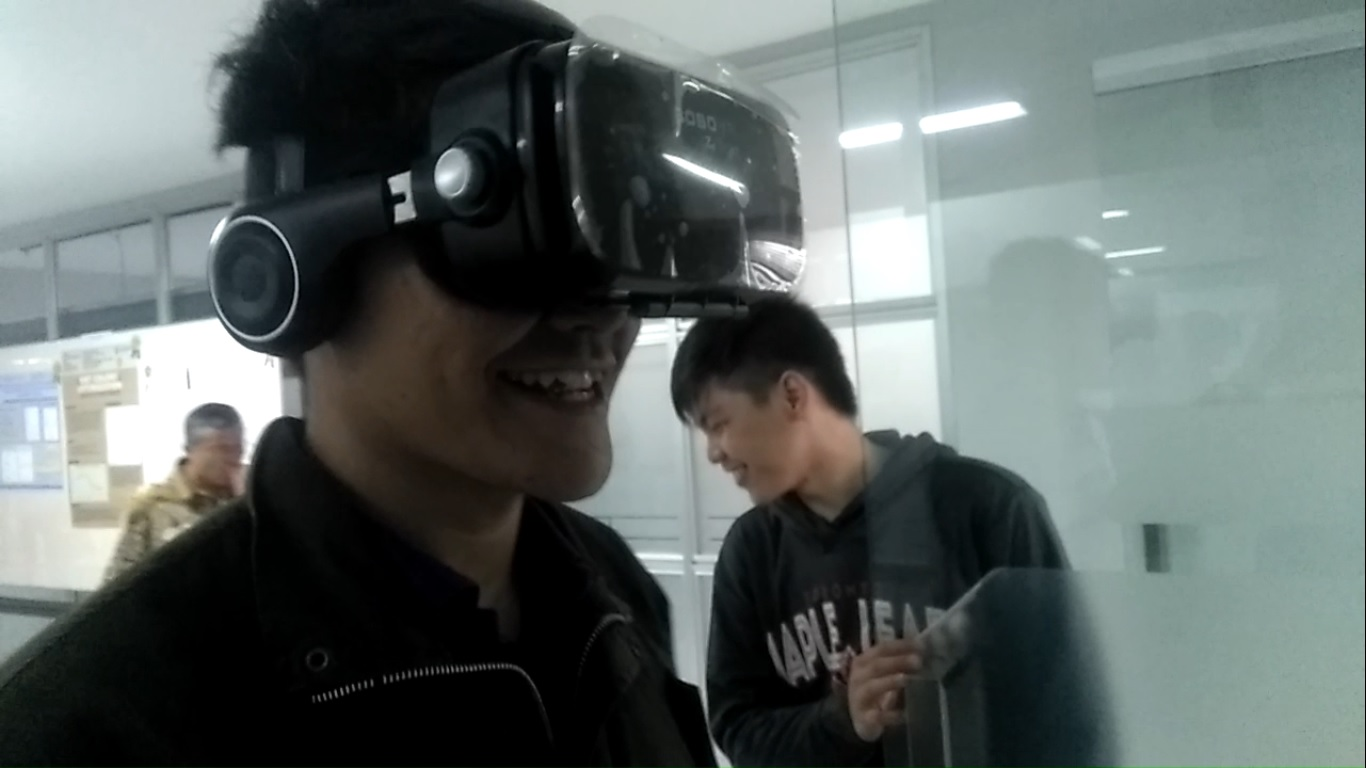
\includegraphics[scale=0.35]{Gambar/PengujianEksperimental/RickySetiawan.jpg}
    \caption{Pengujian oleh Ricky Setiawan.} 
    \label{fig:pengujian_ricky_setiawan}
    \end{figure}
    
    \item Harseto Pandityo (Gambar \ref{fig:pengujian_harseto_pandityo}) menggunakan perangkat \textit{smartphone} nomor 3\\
    "Permainannya bagus dan menarik, khususnya pada fungsi mengangguk dengan menggeleng. Terkadang ada masalah ketika mengangguk tidak terdeteksi, tetapi harus mengangguk dengan lebih jauh lagi simpangan-nya agar dapat terdeteksi. Tidak ada masalah pada saat menggeleng."
    
    \begin{figure}[htbp]
    \centering
    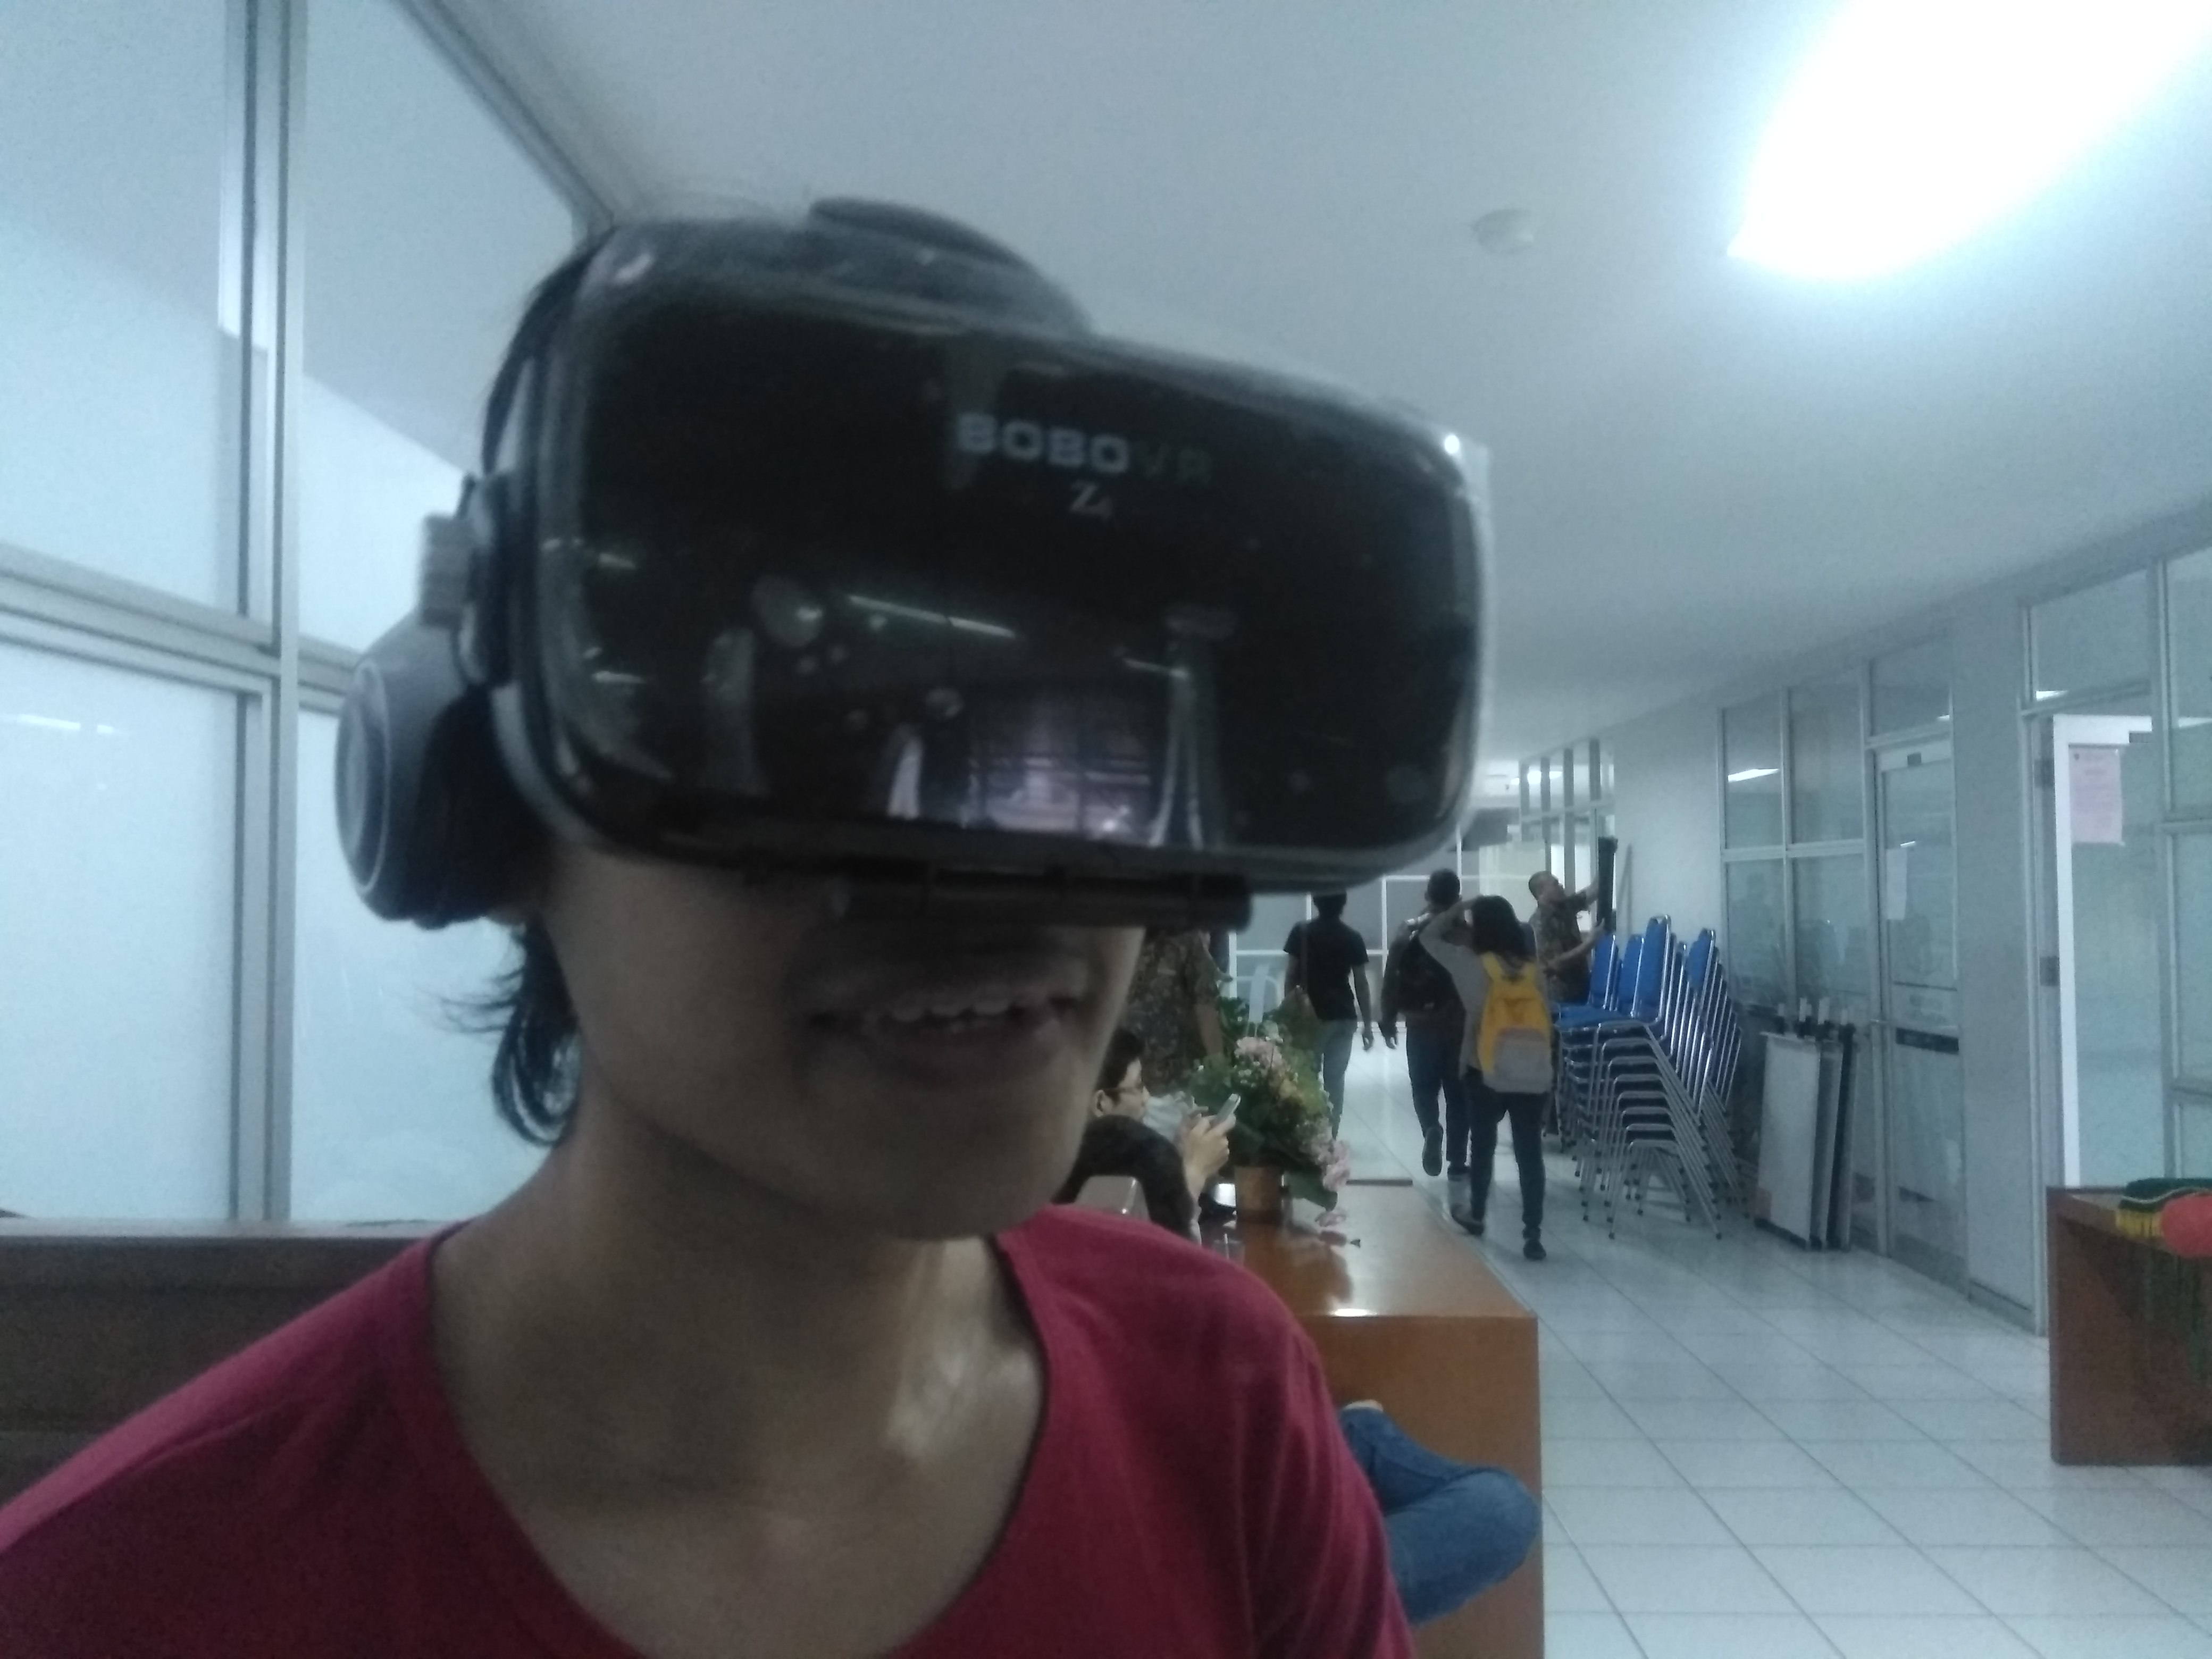
\includegraphics[scale=0.07]{Gambar/PengujianEksperimental/HarsetoPandityo.jpg}
    \caption{Pengujian oleh Harseto Pandityo.} 
    \label{fig:pengujian_harseto_pandityo}
    \end{figure}
    
    \item Herfan Heryandi (Gambar \ref{fig:pengujian_herfan_heryandi}) menggunakan perangkat \textit{smartphone} nomor 5\\
    "Untuk geleng sedikit kurang sensitif, tetapi untuk mengangguk sudah sensitif."

    \begin{figure}[htbp]
    \centering
    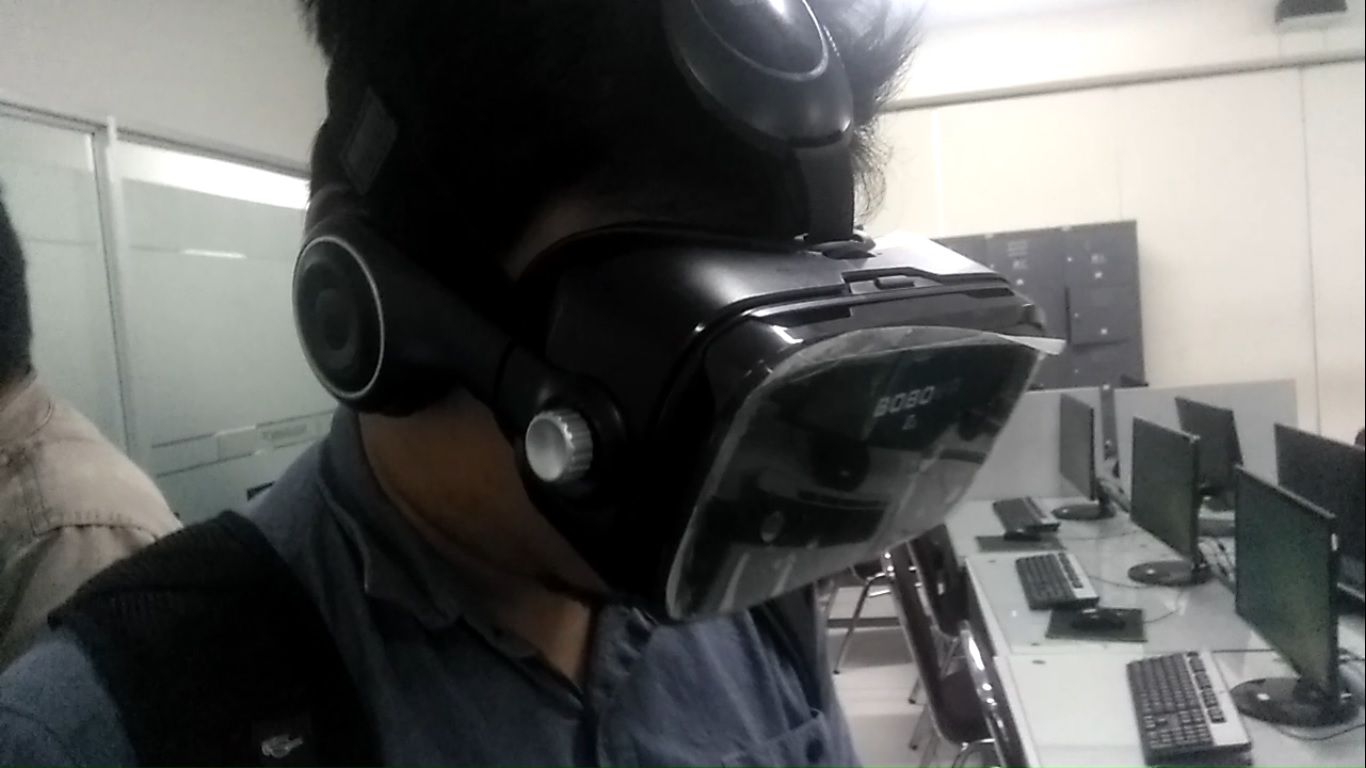
\includegraphics[scale=0.35]{Gambar/PengujianEksperimental/HerfanHeryandi.jpg}
    \caption{Pengujian oleh Herfan Heryandi.} 
    \label{fig:pengujian_herfan_heryandi}
    \end{figure}
    
    \item Kevin Antonius (Gambar \ref{fig:pengujian_kevin_antonius}) menggunakan perangkat \textit{smartphone} 3\\
    
    "Udah bagus, terkadang ketika mengangguk tidak terdeteksi. Mungkin karena anggukan saya terlalu kecil simpangannya."
    
    \begin{figure}[htbp]
    \centering
    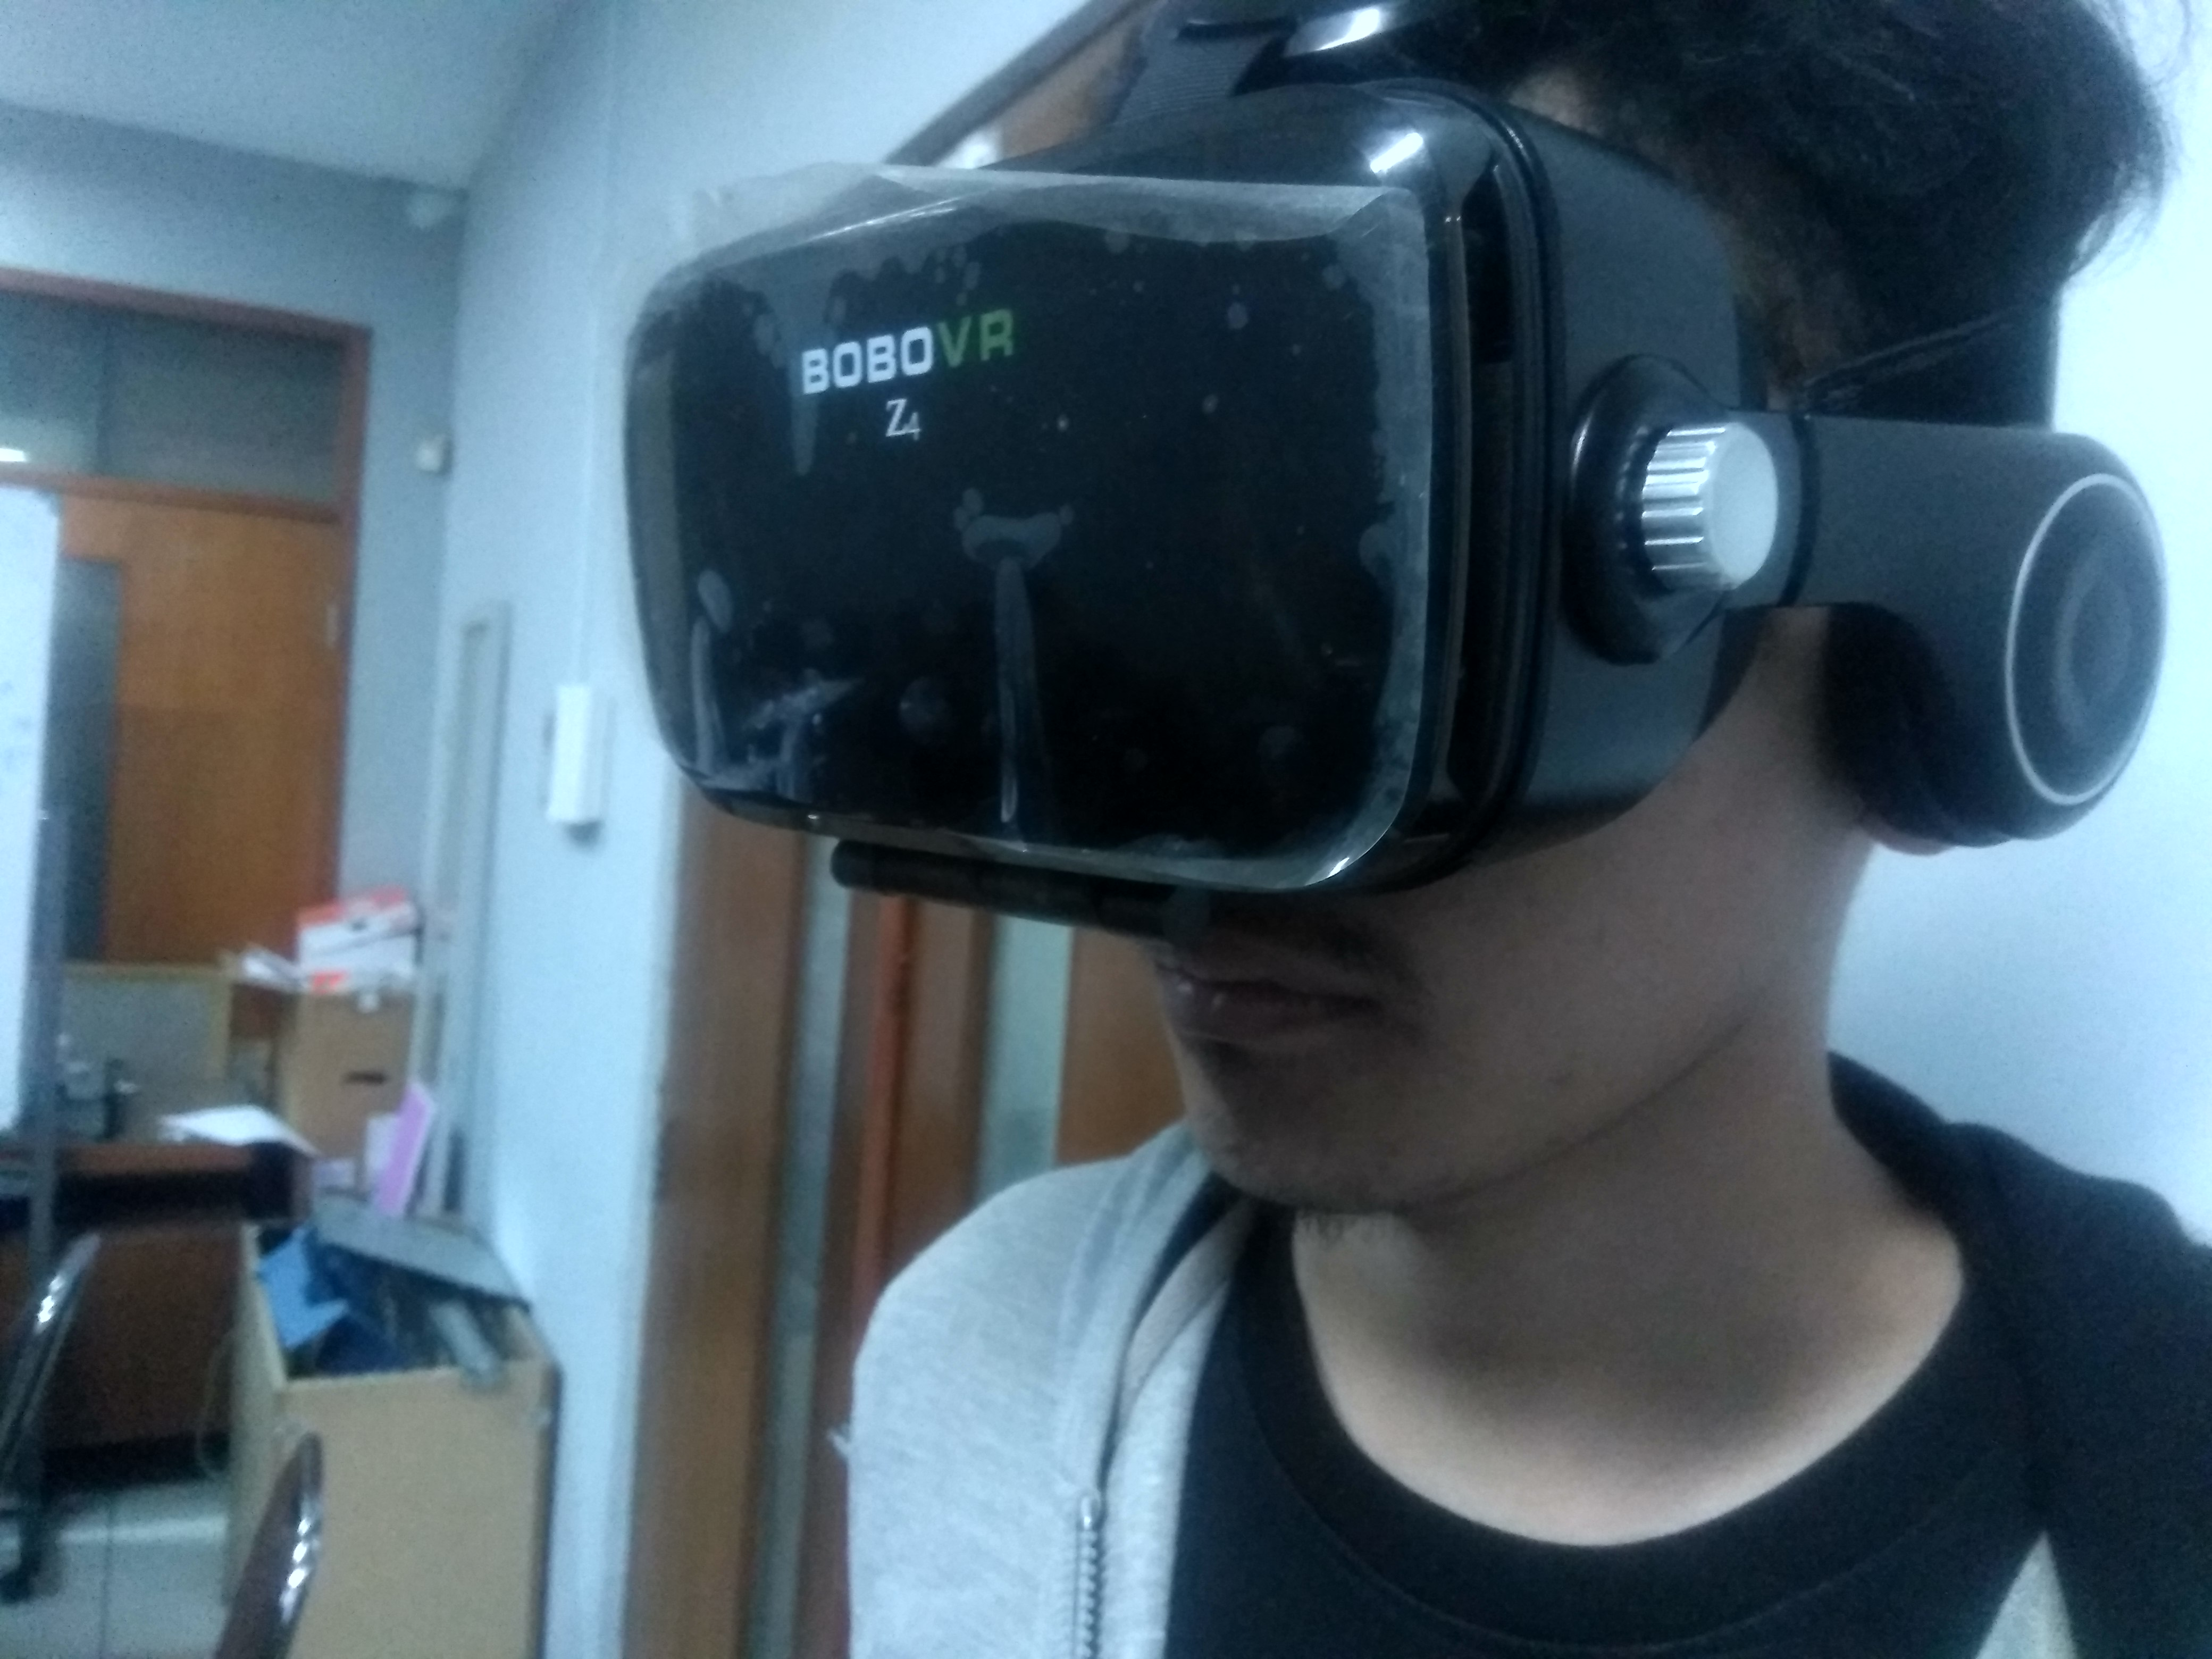
\includegraphics[scale=0.07]{Gambar/PengujianEksperimental/KevinAntonius.jpg}
    \caption{Pengujian oleh Kevin Antonius.} 
    \label{fig:pengujian_kevin_antonius}
    \end{figure}
    
    \item Antonius Kurnia (Gambar \ref{fig:pengujian_antonius_kurnia}) menggunakan perangkat \textit{smartphone} 3\\
    
    "Sensor untuk deteksinya sudah bagus, sudah dapat mendeteksi anggukan dan gelengan dengan baik. Hanya saja terkadang susah membaca tulisannya, karena gerakan anggukan dan gelengannya"
    
    \begin{figure}[htbp]
    \centering
    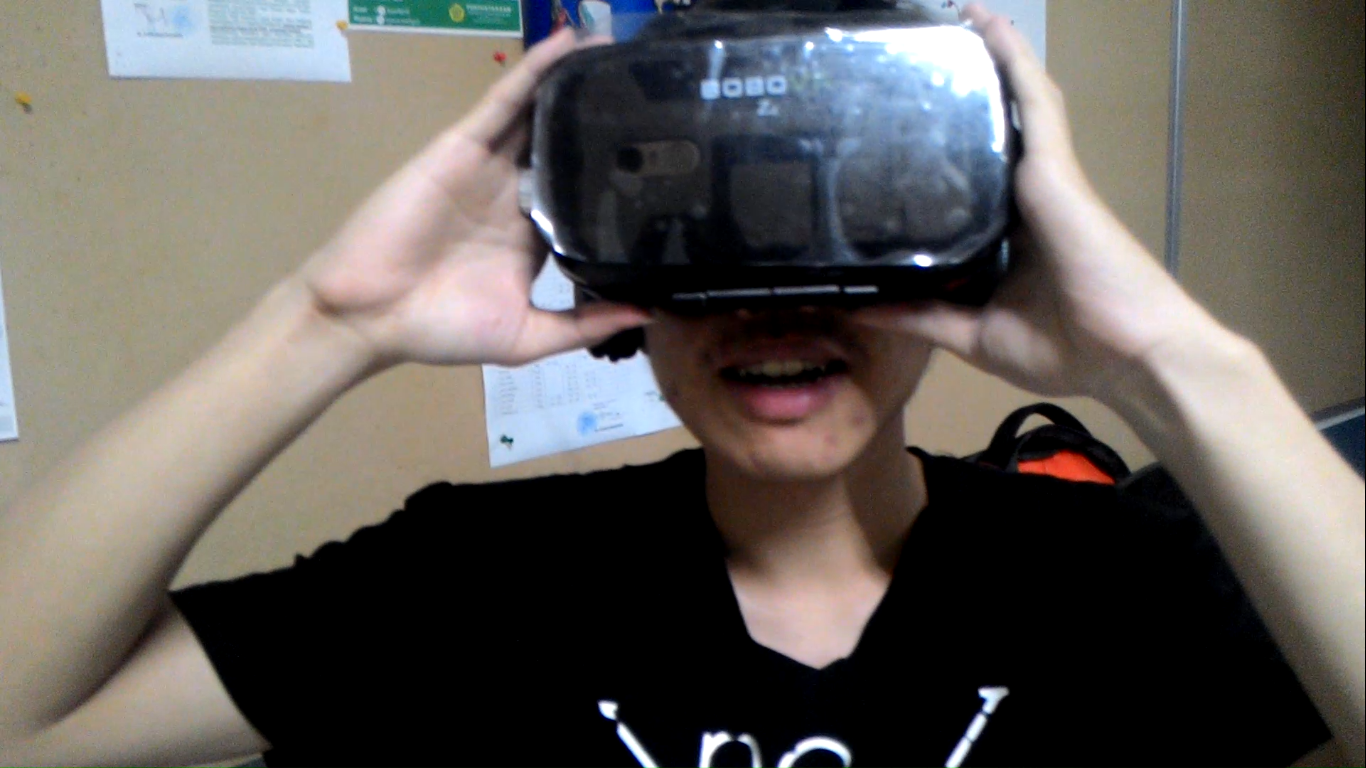
\includegraphics[scale=0.3]{Gambar/PengujianEksperimental/AntoniusKurnia.png}
    \caption{Pengujian oleh Antonius Kurnia.} 
    \label{fig:pengujian_antonius_kurnia}
    \end{figure}
    
\end{enumerate}

\section{Masalah yang Dihadapi pada Saat Implementasi}

Berikut adalah beberapa masalah yang dihadapi pada saat implementasi:
\begin{enumerate}
    \item Sulit dalam mencari permainan \textit{open source} yang telah ada. Rencana awal dalam mengimplementasi algoritma ini adalah dengan mencari permainan \textit{open source} yang telah ada, namun permainan \textit{open source} yang telah mengimplementasi Google VR sangatlah langka. Ketika telah menemukan permainan \textit{open source} yaitu "Doom VR", SDK yang digunakan oleh permainan merupakan SDK dengan versi lama yang sudah tidak dikembangkan lagi oleh Google. Sehingga peneliti tidak dapat menemukan SDK Google VR versi lama. Jadi masalah ini diselesaikan dengan membuat suatu game baru dengan bantuan Game Engine Unity.
    \item Penggunaan Quaternion untuk menyimpan orientasi GameObject-GameObject pada Unity membuat bingung pada saat implementasi. Hal ini terjadi karena penggunaan Quaternion yang di konversi menjadi sudut Euler membuat objek tersebut tidak dapat menyimpan sudut putar yang lebih besar dari 360 derajat dan lebih kecil dari 0 derajat.
    \item Google VR for Unity belum sepenuhnya stabil. Pada saat instalasi Google VR for Unity terjadi \textit{compile error}. Kesalahan \textit{compile error} ini tidak diberikan penyelesaiannya pada website resmi Google VR maupun Unity. Sehingga saya mencari solusi-nya pada forum pengguna Unity. Satu-satunya solusi untuk menyelesaikan solusi ini adalah dengan mengganti satu baris kode pada Google VR for Unity. \textit{Compile error} tersebut terjadi pada script C\# "GvrVideoPlayerTexture.cs" pada baris 595. Solusinya yaitu dengan menambahkan kode "   yield break;" sebelum perintah "return;". Sekarang masalah ini sudah diperbaiki oleh Google VR sehingga tidak terjadi lagi.
\end{enumerate}